% questions.tex —— 2015 年·四川卷·文科 · 题目内容片段（无答案）
% 由 tools/generate_projects.py 依来源总账自 2015/2015_数学真题_四川文_试题.md 生成，勿手改（改源 MD 后重跑）


\gkpart{数学}

\begin{gktip}
\textbf{来源说明}：本题面依据固定源 PDF 全 2 页逐题核对（p1＝页 983：栏 1 标题与「一、选择题」1–5 与第 6 题框图与 7；栏 2 8–10＋「二、填空题」11–15＋「三、解答题」16；栏 3 第 17 题（含座位表）与第 18 题（含两幅图）；p2＝页 984：栏 1 解答 19、栏 2 解答 20（含椭圆图）、栏 3 解答 21）。原卷为 \textbf{A3 横向（1190.55 \(\times\) 841.89 pt）三栏书刊合排}，阅读序＝左→中→右；\textbf{页脚仅印合订本书页页码 983／984}（页面底部正中，x 587.40–603.15 pt），\textbf{无页眉}。标题「2015 普通高等学校招生考试（四川卷文）」在栏 1 内排印。\textbf{全卷不印分值、不印题量、不印「考生注意」栏}——三处节头逐字仅「一、选择题」「二、填空题」「三、解答题」，解答题无「（本小题满分 N 分）」行；总分 150 为结构推断，\textbf{卷面无凭据}，本文件不作补写。

\textbf{源制作体系判定}（\texttt{pdffonts}／\texttt{pdftotext -layout}／\texttt{pdfimages -list} 实测）：源\textbf{不是扫描件，而是 LaTeX（Computer Modern 系）重排产物}——\texttt{pdfimages -list} 零命中（全页无位图；p1 98 条路径＝91 描边＋7 纯填充箭头，p2 12 条路径＝10 描边＋2 纯填充箭头）；嵌入字体含中文 \textbf{STSong（宋体正文）／STHeiti（黑体标题与节头）}，拉丁与数学 \textbf{LMRoman 系与 CM 系（CMR10／CMMI10／CMSY10／CMR7／CMSY7／CMMI7／CMEX10／MSAM10／CMMIB10）}，另有 \textbf{TeX-vect10}（专供第 20 题向量符号绘制）。文本层整体可读；根号上划线、作答空线、表线、全部箭头与向量符号均为矢量路径。

\textbf{标点与字样约定（实测）}：① \textbf{题号与句末}源内为半角 \texttt{.}（LMRoman10 出字），按全库约定写作全角「．」；② \textbf{正文句读}源内为半角 ASCII（\texttt{, : ; ?}）与半角圆括号，本文件按全库约定归一为全角「，」「：」「；」「？」「（）」，\textbf{顿号「、」与引号「“”」为全角 CJK·照源保留}，内容零改动（逐处替换台账见工作档 \texttt{transcripts/partB.md}）；③ \textbf{选择题选项标号}源内为\textbf{半角「(A)」照录}；④ \textbf{作答空}：填空题统一长度横线（实测 31.4883 pt，写作 \texttt{\gkblank{}}），选择题作答括注按全库约定写作「（　）」；⑤ \textbf{分数}源内均为显示风格（真分式），排印一律按显示风格（如 \(\dfrac{a}{b}\)）；⑥ \textbf{不等号}按 MSAM10 实测字形排 \(\leqslant\)／\(\geqslant\)；⑦ \textbf{向量}：第 2 题的 \(\boldsymbol{a}\)、\(\boldsymbol{b}\) 源为\textbf{粗斜体}（CMMIB10），录作 \(\boldsymbol{a}\)／\(\boldsymbol{b}\)；第 20 题的 \(\overrightarrow{PC}\) 类源为 \textbf{TeX-vect10 矢量绘制}（文本层呈干扰字符），按语义排印 \(\overrightarrow{PC}\cdot\overrightarrow{PD}\)；⑧ \textbf{常数与函数名}：\(\mathrm{e}\)（第 8 题）与 \(\lg\)、\(\log\)、\(\sin\)、\(\cos\) 源为\textbf{正体}（LMRoman10），录作 \(\mathrm{e}\)、\(\lg\) 等；温度度号源为 CMSY7 的 \(\circ\)，录作 \(^{\circ}\mathrm{C}\)；⑨ \textbf{第 9 题不等式组}源为\textbf{行内竖排三行}（与整句同行），本文件照源以行内 \texttt{cases} 录入（无对齐 \texttt{\&}）；⑩ \textbf{第 17 题座位表}源为\textbf{全框线表格}（6 横线＋35 竖线逐格绘制，最左列「乘客」在上格、「座位号」纵跨 4 行），本文件照源\textbf{保留全框线}以行间 \texttt{array} 录入（先例：2004 全国Ⅱ理第 13 题、2014 全国Ⅱ文第 19 题），「座位号」简化为数据首行首格（源为纵跨合并格，语义等价）；⑪ \textbf{词间空格}照页面词界补。

\textbf{存疑与登记}（源内异常一律照录；完整清单见工作档 \texttt{figure-inventory.md} 存疑表 S-1…S-7）：① \textbf{固定源不附参考答案}（等级 D）——本题面无答案区，解析全部由本库独立推导；② \textbf{第 18 题展开图与直观图的 A–E 标注互为镜像}——按「字母朝外折叠」约定枚举正方体全部 24 个旋转无相符标法，须按「以图中 A–E 标注定标」（等价于字母朝内折叠）理解；两幅图\textbf{照源复刻}，第 (1) 问的 F/G/H 落点由拓扑唯一确定（不受镜像影响）；③ \textbf{第 20 题椭圆图割线未精确过 P(0,1)}——割线与 y 轴交点实测在原点上方 1.0686 单位（按题意为 1.0000 单位，差 1.94 pt）；图意显系「过 P 的动直线」，\textbf{照源复刻}（割线两端点照实测坐标）；④ \textbf{第 18 题右幅直观图非严格斜二测}——前面实测 68.01 \(\times\) 64.12 pt（宽高比 1.0607），纵向被压缩 5.72\%，系源重排产物特征，\textbf{照源实测复刻}；⑤ \textbf{第 17 题表最左列无斜线}——「乘客」「座位号」为上下堆叠（乘客在上格、座位号纵跨 4 行），非斜格表头；⑥ 「（写出所有真命题的序号）」等三处说明性括注照源（源为半角，已按全库约定归一全角）；⑦ 全卷无分值印制，不录不补。
\end{gktip}

\gkpart{试题}

\gkpart{一、选择题}

\begin{question}
\gkti{1}设集合 \(A=\{x\mid -1<x<2\}\)，集合 \(B=\{x\mid 1<x<3\}\)，则 \(A\cup B=\)（　）

(A) \(\{x\mid -1<x<3\}\)　(B) \(\{x\mid -1<x<1\}\)

(C) \(\{x\mid 1<x<2\}\)　(D) \(\{x\mid 2<x<3\}\)

\end{question}
\begin{question}
\gkti{2}设向量 \(\boldsymbol{a}=(2,4)\) 与向量 \(\boldsymbol{b}=(x,6)\) 共线，则实数 \(x=\)（　）

(A) 2　(B) 3　(C) 4　(D) 6

\end{question}
\begin{question}
\gkti{3}某学校为了了解三年级、六年级、九年级这三个年级之间的学生视力是否存在显著差异，拟从这三个年级中按人数比例抽取部分学生进行调查，则最合理的抽样方法是（　）

(A) 抽签法　(B) 系统抽样法　(C) 分层抽样法　(D) 随机数法

\end{question}
\begin{question}
\gkti{4}设 \(a,b\) 为正实数，则“\(a>b>1\)”是“\(\log_2 a>\log_2 b>0\)”的（　）

(A) 充要条件　(B) 充分不必要条件

(C) 必要不充分条件　(D) 既不充分也不必要条件

\end{question}
\begin{question}
\gkti{5}下列函数中，最小正周期为 \(\pi\) 的奇函数是（　）

(A) \(y=\sin\left(2x+\dfrac{\pi}{2}\right)\)　(B) \(y=\cos\left(2x+\dfrac{\pi}{2}\right)\)

(C) \(y=\sin 2x+\cos 2x\)　(D) \(y=\sin x+\cos x\)

\Needspace{0.4\textheight}
\end{question}
\begin{question}
\gkti{6}执行如图所示的程序框图，输出 \(S\) 的值为（　）
\nopagebreak[4]
\begin{center}% 第 6 题程序框图：按固定源内容流矢量层精确值复刻（1 pt → 0.03515 cm，与全库同制）。
% 原点取框图竖轴 x=216.1406 pt、底缘（结束框底）y（顶向下）=688.7070 pt；y 向上。
% 源实测（figure-inventory §1）：竖轴严格 x=216.1406；7 框（开始=圆角 27.988×16.832、
% k=1 矩形 32.035×14.285、k=k+1 矩形 50.660×15.160、k>4? 菱形 76.008×18.879、
% S=sin(kπ/6) 矩形 57.219×28.586（内嵌真分式故双倍高）、输出 S 平行四边形（斜偏 6.133）、
% 结束=圆角 27.988×17.008）；连线 6 竖直（x=0）+「否」支 3 段回折（自菱形右顶点右行、
% 上行、左行，箭尖 (0,162.1992) 恰落于 k=1 框与 k=k+1 框之间竖线的中点——回流到 k=k+1 之前）；
% 全图无虚线、除 7 支实心箭头外无填充；框内文字 STSong/CM 系 10.5 pt，本图用 \small 同制。
\begin{tikzpicture}[x=0.03515cm,y=0.03515cm,>=stealth,every node/.style={font=\small,inner sep=0pt}]
% ===== 7 框（外轮廓照源实测值）=====
\draw[line width=0.398bp,rounded corners=0.1399cm] (-13.9922,198.3359) rectangle (13.9961,215.1679);  % 1 开始
\draw[line width=0.398bp] (-16.0156,169.4843) rectangle (16.0196,183.7695);                            % 2 k=1
\draw[line width=0.398bp] (-25.3281,139.7578) rectangle (25.3321,154.9179);                            % 3 k=k+1
\draw[line width=0.398bp] (0,125.1093)--(38.0039,115.6679)--(0,106.2304)--(-38.0039,115.6679)--cycle;   % 4 菱形 k>4?
\draw[line width=0.398bp] (-28.6093,62.9961) rectangle (28.6094,91.5820);                              % 5 S=sin(kπ/6)
\draw[line width=0.398bp] (-25.3984,31.5742)--(-19.2656,48.4297)--(25.3945,48.4297)--(19.2617,31.5742)--cycle; % 6 输出 S
\draw[line width=0.398bp,rounded corners=0.1399cm] (-13.9922,0) rectangle (13.9961,17.0078);            % 7 结束
% ===== 连线（6 竖直 + 1 回折；箭尖照源落在下一框边线上）=====
\draw[->,line width=0.398bp] (0,198.1367)--(0,183.9687);   % 开始→k=1
\draw[->,line width=0.398bp] (0,169.2851)--(0,155.1172);   % k=1→k=k+1（回折靶线）
\draw[->,line width=0.398bp] (0,139.5586)--(0,125.3906);   % k=k+1→菱形顶
\draw[->,line width=0.398bp] (0,105.9492)--(0,91.7812);    % 菱形底→S=sin（是支）
\draw[->,line width=0.398bp] (0,62.7968)--(0,48.6289);     % S=sin→输出 S
\draw[->,line width=0.398bp] (0,31.3750)--(0,17.2070);     % 输出 S→结束
\draw[->,line width=0.398bp] (38.2852,115.6679)--(52.4531,115.6679)--(52.4531,162.1992)--(0,162.1992); % 否支回折（回流 k=k+1 入线中点）
% ===== 框内文字与分支标签（照源字形中心定位）=====
\node at (0,207.2570) {开始};
\node at (0,175.5170) {\(k=1\)};
\node at (0,146.6540) {\(k=k+1\)};
\node at (0,114.6860) {\(k>4?\)};
\node at (0,76.7790) {\(S=\sin\dfrac{k\pi}{6}\)};
\node at (0,40.4740) {输出 \(S\)};
\node at (0,8.9590) {结束};
\node at (-8.8666,99.4340) {是};
\node at (38.3814,124.5270) {否};
\end{tikzpicture}
\end{center}
\nopagebreak[4]
(A) \(-\dfrac{\sqrt{3}}{2}\)　(B) \(\dfrac{\sqrt{3}}{2}\)　(C) \(-\dfrac{1}{2}\)　(D) \(\dfrac{1}{2}\)

\end{question}
\begin{question}
\gkti{7}过双曲线 \(x^2-\dfrac{y^2}{3}=1\) 的右焦点且与 \(x\) 轴垂直的直线，交该双曲线的两条渐近线于 \(A,B\) 两点，\(|AB|=\)（　）

(A) \(\dfrac{4\sqrt{3}}{3}\)　(B) \(2\sqrt{3}\)　(C) \(\sqrt{6}\)　(D) \(4\sqrt{3}\)

\end{question}
\begin{question}
\gkti{8}某食品的保鲜时间 \(y\)（单位：小时）与储藏温度 \(x\)（单位：\(^{\circ}\mathrm{C}\)）满足函数关系 \(y=\mathrm{e}^{kx+b}\)（\(\mathrm{e}=2.718\cdots\) 为自然对数的底数，\(k,b\) 为常数）．若该食品在 \(0^{\circ}\mathrm{C}\) 的保鲜时间是 192 小时，在 \(22^{\circ}\mathrm{C}\) 的保鲜时间是 48 小时，则该食品在 \(33^{\circ}\mathrm{C}\) 的保鲜时间是（　）

(A) 16 小时　(B) 20 小时　(C) 24 小时　(D) 28 小时

\end{question}
\begin{question}
\gkti{9}设实数 \(x,y\) 满足 \(\begin{cases}2x+y\leqslant 10,\\ x+2y\leqslant 14,\\ x+y\geqslant 6,\end{cases}\) 则 \(xy\) 的最大值为（　）

(A) \(\dfrac{25}{2}\)　(B) \(\dfrac{49}{2}\)　(C) 12　(D) 16

\end{question}
\begin{question}
\gkti{10}设直线 \(l\) 与抛物线 \(y^2=4x\) 相交于 \(A,B\) 两点，与圆 \((x-5)^2+y^2=r^2\)（\(r>0\)）相切于点 \(M\)，且 \(M\) 为线段 \(AB\) 的中点．若这样的直线 \(l\) 恰有 4 条，则 \(r\) 的取值范围是（　）

(A) \((1,3)\)　(B) \((1,4)\)　(C) \((2,3)\)　(D) \((2,4)\)

\end{question}
\gkpart{二、填空题}

\begin{question}
\gkti{11}设 \(\mathrm{i}\) 是虚数单位，则复数 \(\mathrm{i}-\dfrac{1}{\mathrm{i}}=\)\gkblank{}．

\end{question}
\begin{question}
\gkti{12}\(\lg 0.01+\log_2 16\) 的值是\gkblank{}．

\end{question}
\begin{question}
\gkti{13}已知 \(\sin\alpha+2\cos\alpha=0\)，则 \(2\sin\alpha\cos\alpha-\cos^2\alpha\) 的值是\gkblank{}．

\end{question}
\begin{question}
\gkti{14}在三棱柱 \(ABC\text{-}A_1B_1C_1\) 中，\(\angle BAC=90^{\circ}\)，其正视图和侧视图都是边长为 1 的正方形，俯视图是直角边的长为 1 的等腰直角三角形．设点 \(M,N,P\) 分别是棱 \(AB,BC,B_1C_1\) 的中点，则三棱锥 \(P\text{-}A_1MN\) 的体积是\gkblank{}．

\end{question}
\begin{question}
\gkti{15}已知函数 \(f(x)=2^x\)，\(g(x)=x^2+ax\)（其中 \(a\in\mathbf{R}\)）．对于不相等的实数 \(x_1,x_2\)，设 \(m=\dfrac{f(x_1)-f(x_2)}{x_1-x_2}\)，\(n=\dfrac{g(x_1)-g(x_2)}{x_1-x_2}\)，现有如下命题：

① 对于任意不相等的实数 \(x_1,x_2\)，都有 \(m>0\)；

② 对于任意的 \(a\) 及任意不相等的实数 \(x_1,x_2\)，都有 \(n>0\)；

③ 对于任意的 \(a\)，存在不相等的实数 \(x_1,x_2\)，使得 \(m=n\)；

④ 对于任意的 \(a\)，存在不相等的实数 \(x_1,x_2\)，使得 \(m=-n\)．

其中的真命题有\gkblank{}．（写出所有真命题的序号）

\end{question}
\gkpart{三、解答题}

\begin{question}
\gkti{16}设数列 \(\{a_n\}\)（\(n=1,2,3,\cdots\)）的前 \(n\) 项和 \(S_n\) 满足 \(S_n=2a_n-a_1\)，且 \(a_1\)，\(a_2+1\)，\(a_3\) 成等差数列．

（1） 求数列 \(\{a_n\}\) 的通项公式；

（2） 记数列 \(\left\{\dfrac{1}{a_n}\right\}\) 的前 \(n\) 项和为 \(T_n\)，求 \(T_n\)．

\end{question}
\begin{question}
\gkti{17}一辆小客车上有 5 个座位，其座位号为 1，2，3，4，5．乘客 \(P_1,P_2,P_3,P_4,P_5\) 的座位号分别为 1，2，3，4，5，他们按照座位号从小到大的顺序先后上车．乘客 \(P_1\) 因身体原因没有坐自己的 1 号座位，这时司机要求余下的乘客按以下规则就座：如果自己的座位空着，就只能坐自己的座位；如果自己的座位已有乘客就座，就在这 5 个座位的剩余空位中任意选择座位．

\Needspace{5\baselineskip}
（1） 若乘客 \(P_1\) 坐到了 3 号座位，其他乘客按规则就座，则此时共有 4 种坐法．下表给出了其中两种坐法，请填入余下两种坐法（将乘客就座的座位号填入表中空格处）；

\nopagebreak[4]
\[
\begin{array}{|c|c|c|c|c|c|}
\hline
\text{乘客} & P_1 & P_2 & P_3 & P_4 & P_5\\
\hline
\text{座位号} & 3 & 2 & 1 & 4 & 5\\
\hline
& 3 & 2 & 4 & 5 & 1\\
\hline
& & & & & \\
\hline
& & & & & \\
\hline
\end{array}
\]

（2） 若乘客 \(P_1\) 坐到了 2 号座位，其他乘客按规则就座，求乘客 \(P_5\) 坐到 5 号座位的概率．

\Needspace{0.4\textheight}
\end{question}
\begin{question}
\gkti{18}一个正方体的平面展开图及该正方体的直观图的示意图如图所示．
\nopagebreak[4]
\begin{center}% 第 18 题正方体平面展开图＋直观图（两幅一体）：按固定源内容流矢量层精确值复刻（1 pt → 0.03515 cm，与全库同制）。
% 原点取展开图左上角 x=917.4062 pt、底缘 y（顶向下）=668.4500 pt（直观图 A/B 标签下缘）；y 向上。
% 源实测（figure-inventory §3）：
% 左幅（展开图）：十字六连方（竖条 1×4 叠横条 3×1 共用中格）；格边长 28.3359；
%   竖条轮廓 x 28.3360–56.6719、y 12.8355–126.3992；横条轮廓 x 0–85.0078、y 69.7273–98.0633；
%   竖条内部第 3 条格线 @ y 41.3914。8 个字母全部贴网格顶点排印（锚点见 figure-inventory §3.1.1）。
% 右幅（直观图）：8 顶点/12 棱（9 实 + 3 虚，虚线节距 2.98883，均自隐藏点 BBL 出发）；
%   前面 68.0117 × 64.1211（非严格斜二测，纵向压缩 5.72%，照源复刻）；深度偏移 (+24.0430, −24.0430)。
% 源内异常（照源复刻、已登记）：展开图与直观图 A–E 标注互为镜像（见试题文件存疑登记②）。
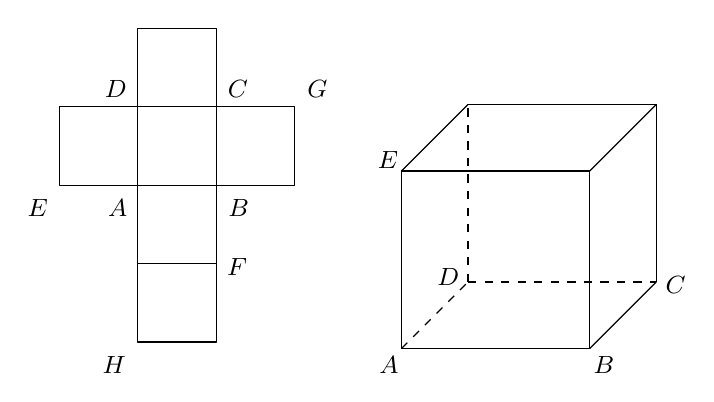
\begin{tikzpicture}[x=0.03515cm,y=0.03515cm,every node/.style={font=\small,inner sep=0pt},
  gl/.style={line width=0.398bp,line join=round}]
% ===== 左幅：平面展开图（十字六连方，格边长 28.3359）=====
\draw[gl] (28.3360,13.0555) rectangle (56.6719,126.3992);   % 竖条外轮廓（1×4）（修复 2026-10-11：下边 12.8355→13.0555＝668.45−655.3945，图自查揪出 0.22pt 传抄误差）
\draw[gl] (0,69.7273) rectangle (85.0078,98.0633);          % 横条外轮廓（3×1）
\draw[gl] (28.3360,41.3914)--(56.6719,41.3914);             % 竖条内部第 3 条格线（R3/R4 分界）
% ===== 左幅字母（照源字形盒中心定位；全部锚于格点）=====
\node at (20.3550,104.2750) {\(D\)};
\node at (64.4900,104.2750) {\(C\)};
\node at (93.2090,104.2750) {\(G\)};
\node at (-7.8340,61.3560) {\(E\)};
\node at (21.0560,61.3560) {\(A\)};
\node at (64.7210,61.3560) {\(B\)};
\node at (64.1150,40.2950) {\(F\)};
\node at (19.7770,4.6620) {\(H\)};
% ===== 右幅：正方体直观图（顶点照源实测）=====
% 实线 9 条
\draw[gl] (123.5430,10.7000)--(191.5547,10.7000);   % 前面下边 A–B
\draw[gl] (191.5547,10.7000)--(215.5977,34.7430);   % 右面下边
\draw[gl] (123.5430,74.8211)--(191.5547,74.8211);   % 前面上边
\draw[gl] (191.5547,74.8211)--(215.5977,98.8641);   % 右面上边
\draw[gl] (215.5977,98.8641)--(147.5860,98.8641);   % 顶面后边
\draw[gl] (147.5860,98.8641)--(123.5430,74.8211);   % 顶面左边
\draw[gl] (191.5547,74.8211)--(191.5547,10.7000);   % 前/右公共竖棱
\draw[gl] (215.5977,98.8641)--(215.5977,34.7430);   % 后面右边
\draw[gl] (123.5430,74.8211)--(123.5430,10.7000);   % 前面左边
% 虚线 3 条（均自隐藏点 BBL 出发；节距照源 2.98883）
\draw[gl,dash pattern=on 2.98883pt off 2.98883pt] (123.5430,10.7000)--(147.5860,34.7430);  % 底面左边（A→隐藏点）
\draw[gl,dash pattern=on 2.98883pt off 2.98883pt] (147.5860,34.7430)--(215.5977,34.7430);  % 底面后边
\draw[gl,dash pattern=on 2.98883pt off 2.98883pt] (147.5860,34.7430)--(147.5860,98.8641);  % 后面左边
% ===== 右幅字母（照源字形盒中心定位）=====
\node at (118.7040,78.6700) {\(E\)};
\node at (140.4790,36.6940) {\(D\)};
\node at (222.6230,33.6440) {\(C\)};
\node at (119.0060,4.6620) {\(A\)};
\node at (196.6420,4.6620) {\(B\)};
\end{tikzpicture}
\end{center}
\nopagebreak[4]
（1） 请将字母 \(F,G,H\) 标记在正方体相应的顶点处（不需说明理由）；

（2） 判断平面 \(BEG\) 与平面 \(ACH\) 的位置关系，并证明你的结论；

（3） 证明：直线 \(DF\perp\) 平面 \(BEG\)．

\end{question}
\begin{question}
\gkti{19}已知 \(A,B,C\) 为 \(\triangle ABC\) 的内角，\(\tan A,\tan B\) 是关于 \(x\) 的方程 \(x^2+\sqrt{3}px-p+1=0\)（\(p\in\mathbf{R}\)）的两个实根．

（1） 求 \(C\) 的大小；

（2） 若 \(AB=3\)，\(AC=\sqrt{6}\)，求 \(p\) 的值．

\Needspace{0.4\textheight}
\end{question}
\begin{question}
\gkti{20}如图，椭圆 \(E:\dfrac{x^2}{a^2}+\dfrac{y^2}{b^2}=1\)（\(a>b>0\)）的离心率是 \(\dfrac{\sqrt{2}}{2}\)，点 \(P(0,1)\) 在短轴 \(CD\) 上，且 \(\overrightarrow{PC}\cdot\overrightarrow{PD}=-1\)．
\nopagebreak[4]
\begin{center}% 第 20 题椭圆图：按固定源内容流矢量层精确值复刻（1 pt → 0.03515 cm，与全库同制）。
% 原点取 x 轴负端 x=616.4024 pt、y 轴下端 y（顶向下）=289.6055 pt；y 向上。
% 源实测（figure-inventory §4）：椭圆中心 (76.5078, 56.6719)、半轴 a=56.6719 / b=40.0664、
% 线宽 0.7967 bp（其余线的 2 倍，全卷唯一加粗——突出二次曲线，照源）；x 轴左端过原点、
% 右至箭尖 +153.0156（左右对称外伸 76.5078，但左端不画箭头、右端画）；y 轴下外伸 56.6719、
% 上至箭尖 +116.1797；过 P 的割线 (13.4882,37.6914)–(104.2734,108.6563) 长 115.23；
% 全图 4 描边 + 2 纯填充箭头，无虚线、无点标记。
% 源内异常（照源复刻、已登记）：割线与 y 轴交点实测在原点上方 60.7337（非 P 的 56.6719，
% 差 1.94 pt）——图意「过 P 的动直线」，照源实测端点抄录。
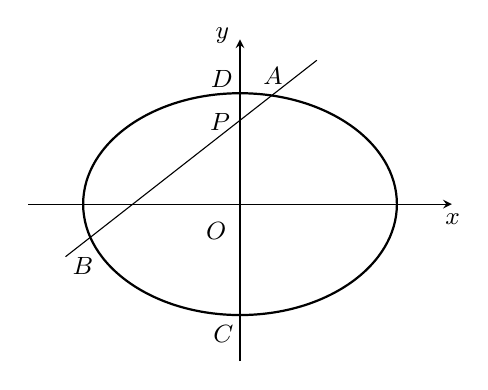
\begin{tikzpicture}[x=0.03515cm,y=0.03515cm,>=stealth,every node/.style={font=\small,inner sep=0pt}]
% ===== 椭圆（4 段贝塞尔，线宽 0.7967 全卷唯一加粗）=====
\draw[line width=0.7967bp] (76.5078,56.6719) ellipse [x radius=56.6719, y radius=40.0664];
% ===== 两轴与箭头 =====
\draw[line width=0.3983bp] (0,56.6719)--(149.4296,56.6719);      % x 轴（右端直线段）
\draw[->,line width=0.3983bp] (149.4296,56.6719)--(153.0156,56.6719); % x 轴箭头（照源独立填充三角，此处并入线端）
\draw[line width=0.3983bp] (76.5078,0)--(76.5078,112.5938);       % y 轴（上端直线段）
\draw[->,line width=0.3983bp] (76.5078,112.5938)--(76.5078,116.1797); % y 轴箭头
% ===== 过 P 的割线 =====
\draw[line width=0.3983bp] (13.4882,37.6914)--(104.2734,108.6563);
% ===== 标签（照源字形盒中心定位）=====
\node at (70.1180,117.6060) {\(y\)};
\node at (88.4580,103.1360) {\(A\)};
\node at (69.9180,101.9860) {\(D\)};
\node at (69.3280,86.1760) {\(P\)};
\node at (153.3080,51.0960) {\(x\)};
\node at (67.9280,47.0060) {\(O\)};
\node at (19.7880,34.4360) {\(B\)};
\node at (70.5480,9.7260) {\(C\)};
\end{tikzpicture}
\end{center}
\nopagebreak[4]
（1） 求椭圆 \(E\) 的方程；

（2） 设 \(O\) 为坐标原点，过点 \(P\) 的动直线与椭圆交于 \(A,B\) 两点．是否存在常数 \(\lambda\)，使得 \(\overrightarrow{OA}\cdot\overrightarrow{OB}+\lambda\overrightarrow{PA}\cdot\overrightarrow{PB}\) 为定值？若存在，求 \(\lambda\) 的值；若不存在，请说明理由．

\end{question}
\begin{question}
\gkti{21}已知函数 \(f(x)=-2x\ln x+x^2-2ax+a^2\)，其中 \(a>0\)．

（1） 设 \(g(x)\) 是 \(f(x)\) 的导函数，讨论 \(g(x)\) 的单调性；

（2） 证明：存在 \(a\in(0,1)\)，使得 \(f(x)\geqslant 0\) 恒成立，且 \(f(x)=0\) 在区间 \((1,+\infty)\) 内有唯一解．

\end{question}